Situs web merupakan salah satu sarana utama dalam penyebaran informasi dan representasi identitas institusi di era digital. Dalam berbagai sektor, termasuk perguruan tinggi, situs web digunakan sebagai kanal resmi untuk menyampaikan informasi secara luas. Perguruan tinggi memanfaatkan situs web untuk menyediakan beragam konten seperti kalender akademik, pengumuman penting, publikasi ilmiah, dokumentasi kegiatan kampus, serta informasi administratif lainnya. Situs web juga menjadi titik awal interaksi antara institusi dengan calon mahasiswa, mitra kerja, media, dan masyarakat umum.

Pentingnya situs web pada perguruan tinggi juga tercermin dari adanya berbagai sistem pemeringkatan non-akademis yang menjadikan situs web resmi perguruan tinggi sebagai objek penilaian. Dua contoh sistem pemeringkatan tersebut adalah Webometrics dan uniRank. Webometrics\footnote{\url{https://webometrics.info} (Diakses pada 7 April 2025)} merupakan sistem pemeringkatan yang dikembangkan oleh Cybermetrics Lab, sebuah kelompok riset di bawah Consejo Superior de Investigaciones Científicas (CSIC) Spanyol. Sistem ini menilai kehadiran dan visibilitas situs web akademik di internet sebagai cerminan dari kinerja dan dampak institusi dalam ranah digital. Namun, sejak April 2025 laman resmi Webometrics sudah tidak dapat diakses. Sementara itu, uniRank\footnote{\url{https://www.unirank.org/about} (Diakses pada 20 Juli 2025)} adalah sistem pemeringkatan yang berfokus pada popularitas dan kehadiran daring situs web perguruan tinggi. Penilaian pada uniRank dilakukan menggunakan empat metrik independen, yaitu \textit{Majestic Referring Domains} (55\%), \textit{Similarweb Global Rank} (35\%), \textit{Moz Domain Authority} (5\%), dan \textit{Majestic Trust Flow} (5\%). \textit{Majestic Referring Domains} mengukur jumlah domain eksternal unik yang memberikan tautan menuju situs web resmi perguruan tinggi, dengan mempertimbangkan kualitas tautan melalui ambang batas \textit{Trust Flow} tertentu. Sementara itu, \textit{Similarweb Global Rank} mencerminkan tingkat popularitas situs berdasarkan estimasi trafik global yang diterima dari berbagai sumber pengunjung. Berdasarkan kedua sistem tersebut, dapat disimpulkan bahwa visibilitas dan pengalaman pengguna merupakan dua aspek yang penting dari situs web perguruan tinggi dan perlu diperhatikan secara berkelanjutan.



Salah satu tantangan dalam menjaga visibilitas dan pengalaman pengguna dalam mengakses situs web perguruan tinggi adalah keberadaan tautan rusak. Tautan rusak terjadi ketika suatu tautan mengarah ke sumber daya yang sudah tidak tersedia atau tidak dapat diakses, sehingga menghasilkan pesan kesalahan seperti \texttt{404 Not Found} atau \texttt{500 Internal Server Error}. Keberadaan tautan rusak dapat menghambat alur navigasi, menurunkan kepercayaan pengguna terhadap isi situs, serta berdampak negatif terhadap peringkat situs dalam mesin pencari dan sistem pemeringkatan daring, seperti uniRank dan Webometrics. Oleh karena itu, pemantauan dan pemeliharaan tautan secara berkala merupakan langkah penting dalam pengelolaan situs web institusi pendidikan tinggi.


Secara umum, terdapat dua pendekatan dalam memeriksa keberadaan tautan rusak pada situs web, yaitu secara manual dan dengan bantuan perangkat lunak. Pemeriksaan manual menjadi tidak praktis ketika situs memiliki ratusan bahkan ribuan halaman. Untuk mengatasi hal ini, tersedia berbagai layanan daring seperti Broken Link Checker\footnote{\url{https://www.brokenlinkcheck.com/} (Diakses pada 20 Juli 2025)}. Broken Link Checker merupakan alat berbasis web yang secara otomatis memindai halaman-halaman dalam sebuah situs web dan mendeteksi tautan rusak di dalamnya. Gambar~\ref{fig:gambar-contoh-brokenlinkcheck} menunjukkan hasil pemindaian pada situs web Informatika UNPAR menggunakan layanan Broken Link Checker, di mana terdeteksi beberapa tautan rusak yang tersebar di berbagai halaman. Dalam laporannya, Broken Link Checker menampilkan informasi penting seperti URL dari tautan rusak yang ditemukan, teks yang menjadi jangkar (\textit{anchor text}) dari tautan tersebut, halaman tempat tautan itu ditemukan, serta respons dari server dalam bentuk kode status HTTP seperti \texttt{404} atau \texttt{500}. Layanan ini juga menyediakan tautan langsung menuju bagian kode sumber tautan rusak ditemukan untuk mempermudah pelacakan lokasi tautan rusak dalam dokumen HTML.

\begin{figure}[H]
    \centering
    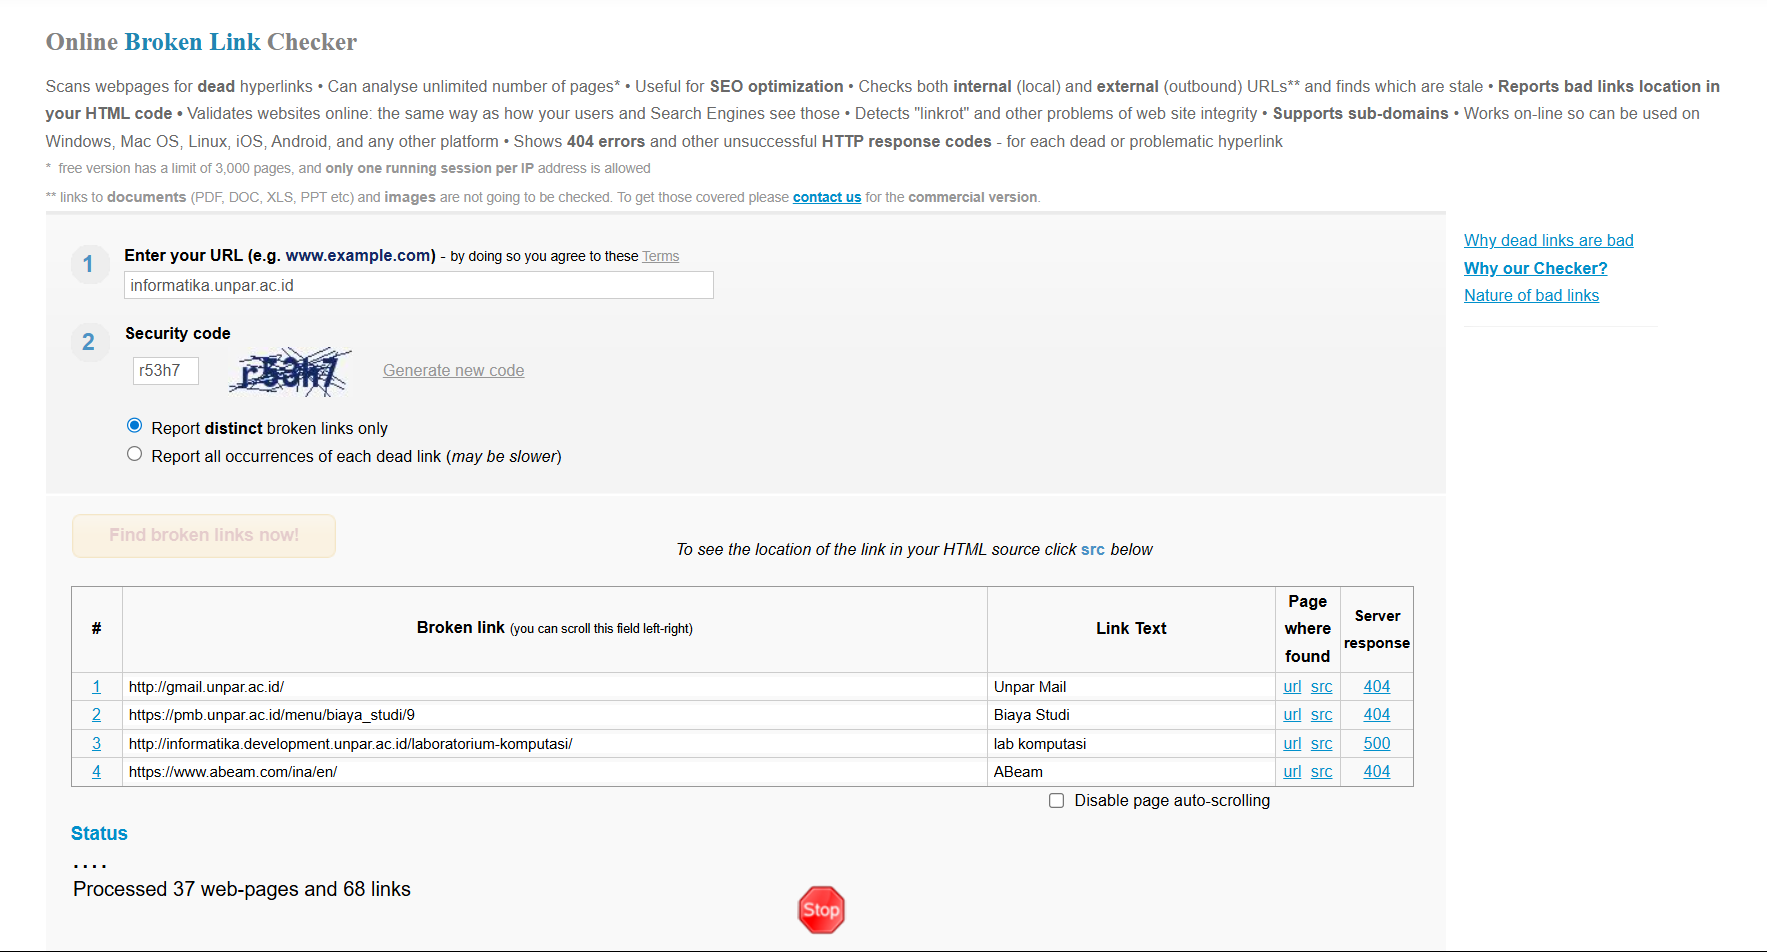
\includegraphics[width=0.85\textwidth]{Gambar/010100-broken-link-checker.png}
    \caption{Tampilan Broken Link Checker}
    \label{fig:gambar-contoh-brokenlinkcheck}
\end{figure}


Dalam penelitian ini akan dikembangkan sebuah perangkat lunak berbasis desktop yang dapat digunakan untuk memeriksa keberadaan tautan rusak pada situs web secara otomatis. Perangkat lunak ini akan menerima masukan berupa alamat situs web, kemudian menelusuri halaman-halaman yang saling terhubung di dalamnya untuk mengidentifikasi seluruh tautan yang terdapat pada situs tersebut. Selanjutnya, setiap tautan akan diperiksa dengan cara mengaksesnya dan mengevaluasi respons yang diberikan oleh server. Berdasarkan hasil pemeriksaan tersebut, perangkat lunak akan menghasilkan laporan yang memuat informasi mengenai tautan-tautan yang terdeteksi rusak. Untuk mempermudah pengguna dalam menjalankan proses pemeriksaan dan membaca hasilnya, perangkat lunak ini juga dilengkapi dengan antarmuka grafis yang intuitif.